% vim: set textwidth=78 autoindent:

% when the revision of a section has been finalized,
% comment out the following line:
%\updatedisclaimer

\section{Vector Spatial Analysis (Buffers)}\label{sec:buffer}
\begin{tabular}{p{3.5cm}p{6cm}p{6cm}}
\multirow{2}{*}{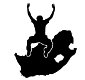
\includegraphics[width=2.5cm]{logo}} & Objectives: &
Understanding the use of buffering in vector spatial analysis. \\
& & \\
& Keywords: & 
Vector, buffer zone, spatial analysis, buffer distance, dissolve boundary,
outward and inward buffer, multiple buffer  \\
\hline
\end{tabular}

\subsection{Overview}

\textbf{Spatial analysis} uses spatial information to extract new and additional
meaning from GIS data. Usually spatial analysis is carried out using a GIS
Application. GIS Applications normally have spatial analysis tools for
feature statistics (e.g. how many vertices make up this polyline?) or
geoprocessing such as feature buffering. The types of spatial analysis that
are used vary according to subject areas. People working in water management
and research (hydrology) will most likely be interested in analysing terrain
and modelling water as it moves across it.  In wildlife management users are
interested in analytical functions that deal with wildlife point locations
and their relationship to the environment. In this topic we will discuss
buffering as an example of a useful spatial analysis that can be carried out
with vector data.

\subsection{Buffering in detail}

\textbf{Buffering} usually creates two areas: one area that is
\textbf{within} a specified distance to selected real world features and the
other area that is \textbf{beyond}. The area that is within the specified
distance is called the \textbf{buffer zone}.

\begin{figure}[ht]
   \begin{center}
   \caption{The border between the United States of America and Mexico is
separated by a buffer zone. (Photo taken by SGT Jim Greenhill 2006).}
\label{fig:mexborder}\smallskip
   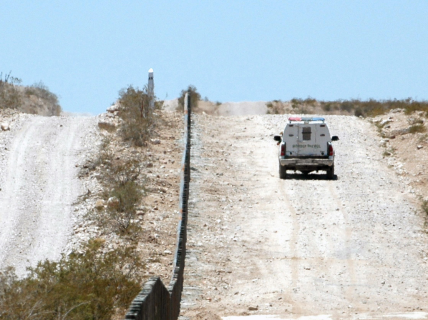
\includegraphics[clip=true, width=0.6\textwidth]{border_usa_mexico}
\end{center}
\end{figure}

A \textbf{buffer zone} is any area that serves the purpose of keeping real world
features distant from one another. Buffer zones are often set up to protect
the environment, protect residential and commercial zones from industrial
accidents or natural disasters, or to prevent violence. Common types of
buffer zones may be greenbelts between residential and
commercial areas, border zones between countries (see Figure
\ref{fig:mexborder}), noise protection zones around airports, or pollution
protection zones along rivers. 

\newpage

In a GIS Application, \textbf{buffer zones} are always represented as
\textbf{vector polygons} enclosing other polygon, line or point features (see
Figures \ref{fig:buffer}a-c). 

\begin{figure}[ht]
\centering
\caption{Buffering vector points, polylines and polygons}\label{fig:buffer}
   \subfigure[A buffer zone around vector points.]
   {\label{subfig:poibuffer}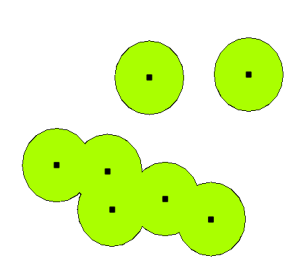
\includegraphics[clip=true, width=0.3\textwidth]{pointbuffer}}\goodgap
   \subfigure[A buffer zone around vector polylines.]
    {\label{subfig:linebuffer}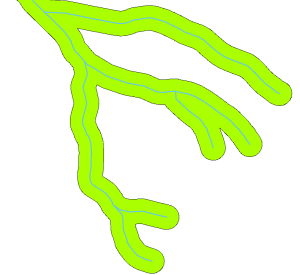
\includegraphics[clip=true, width=0.3\textwidth]{polylinebuffer}}\goodgap
   \subfigure[A buffer zone around vector polygons]
    {\label{subfig:polybuffer}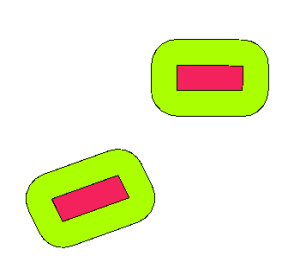
\includegraphics[clip=true, width=0.3\textwidth]{polygonebuffer}}
\end{figure}

\subsection{Variations in buffering}

There are several variations in buffering. The \textbf{buffer distance} or
buffer size \textbf{can vary} according to numerical values provided in the
vector layer attribute
table for each feature. The numerical values have to be defined in map units
according to the Coordinate Reference System (CRS) used with the data.  For
example, the width of a buffer zone along the banks of a river can vary
depending on the intensity of the adjacent land use. For intensive
cultivation the buffer distance may be bigger than for organic farming (see
Figure \ref{fig:riverbuffer} and Table \ref{tab:buffer}).

\begin{figure}[ht]
   \begin{center}
   \caption{Buffering rivers with different buffer distances.}
\label{fig:riverbuffer}\smallskip
   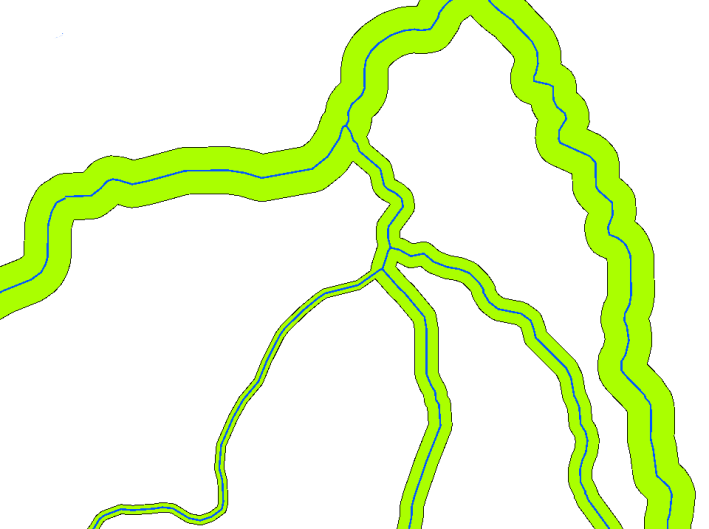
\includegraphics[clip=true, width=0.5\textwidth]{variable_buffer}
\end{center}
\end{figure}

%% Note: xdvi does not show white text on black background but it works!
\begin{table}[ht]
\centering
\caption{Attribute table with different buffer distances to rivers based on
information about the adjacent land use.}\medskip
 \label{tab:buffer}
 \begin{tabular}{|p{5cm}|p{6cm}|p{5cm}|}
 \hline
 \rowcolor{black}
 \textcolor{white}{\textbf{River}} &
 \textcolor{white}{\textbf{Adjacent land use}} &
 \textcolor{white}{\textbf{Buffer distance (meters)}} \\
 \hline Breede river & Intensive vegetable cultivation & 100 \\
 \hline Komati & Intensive cotton cultivation & 150 \\
 \hline Oranje & Organic farming & 50 \\
 \hline Telle river & Organic farming & 50 \\
\hline
\end{tabular}
\end{table}

Buffers around polyline features, such as rivers or roads, do not have to be
on both sides of the lines. They can be on either the left side or the right
side of the line feature. In these cases the left or right side is determined
by the direction from the starting point to the end point of line during
digitising.  

\subsection{Multiple buffer zones}

A feature can also have more than one buffer zone. A nuclear power plant may
be buffered with distances of 10, 15, 25 and 30 km, thus forming multiple
rings around the plant as part of an evacuation plan (see Figure
\ref{fig:powerplant}).  

\begin{figure}[ht]
   \begin{center}
   \caption{Buffering a point feature with distances of 10, 15, 25 and 30 km.}
\label{fig:powerplant}\smallskip
   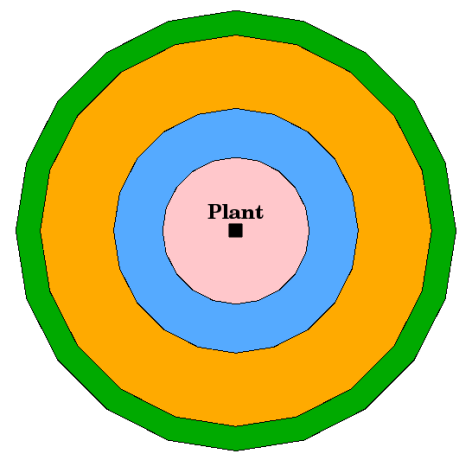
\includegraphics[clip=true, width=0.4\textwidth]{multiple_buffer}
\end{center}
\end{figure}

\subsection{Buffering with intact or dissolved boundaries}

Buffer zones often have dissolved boundaries so that there are no overlapping
areas between the buffer zones. In some cases though, it may also be useful
for boundaries of buffer zones to remain intact, so that each buffer zone is
a separate polygon and you can identify the overlapping areas (see Figure
\ref{fig:buffertypes}).

\begin{figure}[ht]
   \begin{center}
   \caption{Buffer zones with dissolved (left) and with intact boundaries
(right) showing overlapping areas.}
\label{fig:buffertypes}\smallskip
   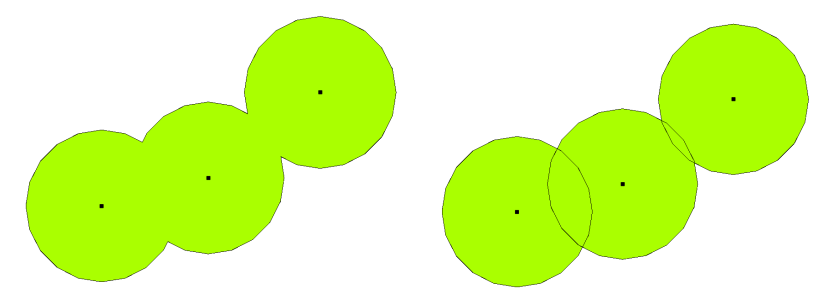
\includegraphics[clip=true, width=0.9\textwidth]{dissolved_intact_buffer}
\end{center}
\end{figure}

\subsection{Buffering outward and inward}

Buffer zones around polygon features are usually extended outward from a
polygon boundary but it is also possible to create a buffer zone inward from
a polygon boundary. Say, for example, the Department of Tourism wants to plan
a new road around Robben Island and environmental laws require that the road
is at least 200 meters inward from the coast line. They could use an inward
buffer to find the 200m line inland and then plan their road not to go beyond
that line.

\subsection{Common problems / things to be aware of}

Most GIS Applications offer buffer creation as an analysis tool, but the
options for creating buffers can vary. For example, not all GIS Applications
allow you to buffer on either the left side or the right side of a line
feature, to dissolve the boundaries of buffer zones or to buffer inward from
a polygon boundary.

A buffer distance always has to be defined as a whole number
(\textbf{integer}) or a decimal number (\textbf{floating point value}). This
value is defined in \textbf{map units} (meters, feet, decimal degrees)
according to the Coordinate Reference System (CRS) of the vector layer. 

\subsection{More spatial analysis tools}

Buffering is a an important and often used spatial analysis tool but there
are many others that can be used in a GIS and explored by the user. 

\begin{figure}[ht]
   \begin{center}
   \caption{Spatial overlay with two input vector layers (a\_input =
rectangle, b\_input = circle). The resulting vector layer is displayed
green.}
\label{fig:overlay}\smallskip
   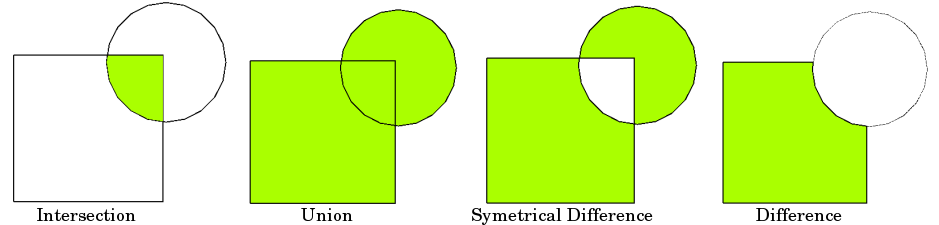
\includegraphics[clip=true, width=\textwidth]{overlay}
\end{center}
\end{figure}

\textbf{Spatial overlay} is a process that allows you to identify the relationships
between two polygon features that share all or part of the same area. The
output vector layer is a combination of the input features information (see
Figure \ref{fig:overlay}). Typical spatial overlay examples are:

\begin{itemize}
\item \textbf{Intersection}: The output layer contains all areas where both
layers overlap (intersect).
\item \textbf{Union}: the output layer contains all areas of the two input
layers combined.
\item \textbf{Symmetrical difference}: The output layer contains all areas of
the input layers except those areas where the two layers overlap (intersect).
\item \textbf{Difference}: The output layer contains all areas of the first
input layer that do not overlap (intersect) with the second input layer.
\end{itemize}

\subsection{What have we learned?}

Let's wrap up what we covered in this worksheet:

\begin{itemize}
\item \textbf{Buffer zones} describe areas around real world features.
\item Buffer zones are always \textbf{vector polygons}.
\item A feature can have \textbf{multiple} buffer zones.
\item The size of a buffer zone is defined by a \textbf{buffer distance}.
\item A buffer distance has to be an \textbf{integer} or \textbf{floating
point} value.
\item A buffer distance can be different for each feature within a vector layer.
\item Polygons can be buffered \textbf{inward} or \textbf{outward} from the
polygon boundary.
\item Buffer zones can be created with \textbf{intact} or \textbf{dissolved}
boundaries.
\item Besides buffering, a GIS usually provides a variety of vector analysis tools
to solve spatial tasks. 
\end{itemize}

\subsection{Now you try!}

\begin{itemize}
\item Because of dramatic traffic increase, the town planners want to widen the
main road and add a second lane. Create a buffer around the road to find
properties that fall within the buffer zone (see Figure \ref{fig:lanebuffer}). 
\item For controlling protesting groups, the police want to establish a neutral
zone to keep protesters at least 100 meters from a building. Create a buffer
around a building and colour it so that event planners can see where the
buffer area is.
\item A truck factory plans to expand. The siting criteria stipulate that a
potential site must be within 1 km of a heavy-duty road. Create a buffer
along a main road so that you can see where potential sites are.
\item Imagine that the city wants to introduce a law stipulating that no bottle
stores may be within a 1000 meter buffer zone of a school or a church. Create
a 1km buffer around your school and then go and see if there would be any
bottle stores too close to your school.
\end{itemize}

\begin{figure}[ht]
   \begin{center}
   \caption{Buffer zone (green) around a roads map (brown). You can see which
houses fall within the buffer zone, so now you could contact the owner and
talk to him about the situation.}
\label{fig:lanebuffer}\smallskip
   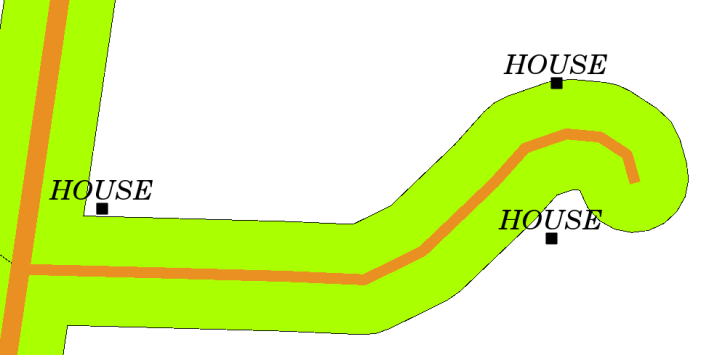
\includegraphics[clip=true, width=0.6\textwidth]{roadbuffer}
\end{center}
\end{figure}

\subsection{Something to think about}

If you don't have a computer available, you can use a toposheet and a compass
to create buffer zones around buildings. Make small pencil marks at equal
distance all along your feature using the compass, then connect the marks
using a ruler!

\subsection{Further reading}

\textbf{Books}: 

\begin{itemize}
\item Galati, Stephen R. (2006): Geographic Information Systems Demystified. Artech
House Inc. (ISBN 158053533X)
\item Chang, Kang-Tsung (2006): Introduction to Geographic Information Systems. 3rd
Edition.  McGraw Hill. (ISBN 0070658986)
\item DeMers, Michael N. (2005): Fundamentals of Geographic Information Systems.
3rd Edition. Wiley. (ISBN 9814126195)
\end{itemize}

\textbf{Websites}:
 
\url{http://www.manifold.net/doc/transform\_border_buffers.htm}

The QGIS User Guide also has more detailed information on analysing vector
data in QGIS.

\subsection{What's next?}

In the section that follows we will take a closer look at
\textbf{interpolation} as an example of spatial analysis you can do with
raster data.


